%%%%%%%%%%%%%%%%%%%%%%%%%%%%%%%%%%%%%%%%%
%%% HYPERRIDE Reporting Template
%%%%%%%%%%%%%%%%%%%%%%%%%%%%%%%%%%%%%%%%%

\documentclass[letterpaper,12pt]{report}
\usepackage[pass]{geometry}
%\documentclass[11pt]{report}

\usepackage{hyperride}		% HYPERRIDE specific definitions and styles  
\usepackage[utf8]{inputenc}	% UTF8 package
\usepackage[T1]{fontenc}
\usepackage{textcomp}		% common special chars
\usepackage{amsmath}		% math formula
\usepackage{fancybox}
\usepackage{anyfontsize}	% fonts
\usepackage{lipsum}
\usepackage{float}
\usepackage[normalem]{ulem}
\usepackage{cleveref}
\usepackage[printonlyused]{acronym}
\hypersetup{
	pdftitle={0th Periodic Report},
	pdfauthor={[Names of co-authors (partners short names)]},
	pdfkeywords={Periodic Report, European Union (EU), H2020, Project, HYPERRIDE, GA 957788},
}
\usepackage{subfigure}
\usepackage{graphicx}
\usepackage{xcolor}
\usepackage{soul}
\sethlcolor{lightgray}
\usepackage[export]{adjustbox}
\usepackage{mdframed}
\usepackage{pdfpages}
\usepackage{comment}
\usepackage{multirow,array}
\def\todo#1{{\color{hyperridered}\textbf{TODO:} ``#1''}}
\def\hyperride{HYPERRIDE}

\graphicspath{ {graphics/} }

%%%%%%%%%%%%%%%%%%%%%%%%%%%%%%%%%%%%%%%%%
%%% Definitions
%%%%%%%%%%%%%%%%%%%%%%%%%%%%%%%%%%%%%%%%%



% CHANGE %'s below to make subsection headings visible/invisible in TOC
%\newcommand{\xsubsubsection}[1]{\subsection{#1}}
%\newcommand{\xsubsubsection}[1]{\subsubsection{#1}}

\begin{document}


\includepdf[pages=1]{./graphics/SIA.pdf}

\mdfdefinestyle{code}{%
    linecolor=black,
    outerlinewidth=2pt,
    %roundcorner=20pt,
    innertopmargin=4pt,
    innerbottommargin=4pt,
    innerrightmargin=4pt,
    innerleftmargin=4pt,
        leftmargin = 4pt,
        rightmargin = 4pt
    backgroundcolor=black!10
    }

\setcounter{tocdepth}{4}
\setcounter{secnumdepth}{4}

%%%%%%%%%%%%%%%%%%%%%%%%%%%%%%%%%%%%%%%%%
%%% URL style same as regular text
%%%%%%%%%%%%%%%%%%%%%%%%%%%%%%%%%%%%%%%%%
	
\urlstyle{same}

%%%%%%%%%%%%%%%%%%%%%%%%%%%%%%%%%%%%%%%%%
%%% Deliverable Information
%%%%%%%%%%%%%%%%%%%%%%%%%%%%%%%%%%%%%%%%%

% Project Meta Information
\ProjectFullTitle{Beacon Network Security Labs: Android State Inference Attacks}
\ProjectAcronym{HYPERRIDE}
\ProjectRefNo{957788}

% Report Number, use either "1", "2", or "3" for the corresponding reporting period
\delivNumber{0}

% Period covered by the report
\delivFrom{dd/mm/yyyy}
\delivTo{dd/mm/yyyy}

% Report Responsible Partner
\delivResponsible{AIT Austrian Institute of Technology (AIT)} 

% Report Version, Contractual and Actual Date, Dissemination Level, Type
\delivVersion{vn.n}
\ContractualDate{dd/mm/yyyy}
\ActualDate{dd/mm/yyyy}

% List of Main Authors (usually from the responsible partner)
\delivAuthor{[Names of co-authors (partners short names)]}

% List of Co-Authors (all other co-authors should be listed here)
\delivFPAuthor{[Names of co-authors (partners short names)]}

% Report Status
\delivStatus{d} %% d = draft, f = final, s = submitted

%%%%%%%%%%%%%%%%%%%%%%%%%%%%%%%%%%%%%%%%%
%%% Change Log
%%%%%%%%%%%%%%%%%%%%%%%%%%%%%%%%%%%%%%%%%

\istChange{dd/mm/yyyy}{v1.0}{Name (Partner short name)}{Draft report template}
\istChange{}{}{}{}

%%%%%%%%%%%%%%%%%%%%%%%%%%%%%%%%%%%%%%%%%
%%% Cover Page
%%%%%%%%%%%%%%%%%%%%%%%%%%%%%%%%%%%%%%%%%

%\makecover

%%%%%%%%%%%%%%%%%%%%%%%%%%%%%%%%%%%%%%%%%
%%% Table of Contents
%%%%%%%%%%%%%%%%%%%%%%%%%%%%%%%%%%%%%%%%%

\clearpage
\fancypagestyle{plain}{}
\settableofcontents
\tableofcontents
\clearpage

%%%%%%%%%%%%%%%%%%%%%%%%%%%%%%%%%%%%%%%%%
%%% Overview
%%%%%%%%%%%%%%%%%%%%%%%%%%%%%%%%%%%%%%%%%

\section*{Overview}\label{sec:work-carried-out}
\addcontentsline{toc}{section}{Overview}

When people think about phishing attacks, many commonly think of emails or fake links that target company email domains. However, a very prevalent form of phishing attacks target mobile devices via instant apps and applications. These applications monitor the root device and infer when to inject an application. 

This exercise will build upon the research paper, \textit{Detecting and Preventing State Inference Attacks} by Possemato et al.$^\text{[\citeauthor{possemato2021preventing}]}$, covering vulnerabilities and strategies surrounding mobile devices. In this lab, you will implement and socially engineer an application to monitor state information of a device and steal user information.

\subsection*{Objectives}

Understand conventional attack strategies on mobile devices and some of the vulnerabilities within Android API’s, how to utilize vulnerable API’s to gather state information about a device and its processes, and how to implement a social engineering application that hijacks an activity and steals user information.

\subsection*{Reading}

This lab is based on a paper by Andrea Possemato, Dario Nisi, and Yanick Fratantonio published in the 2021 Network and Distributed System Security (NDSS) Symposium $^\text{[\citeauthor{possemato2021preventing}]}$. Reading the original paper is not neccessary but can help if you would like to learn more about this attack and defense.

A. Possemato, D. Nisi and Y. Fratantonio, "Preventing and Detecting State Inference Attacks on Android", 2021.$^\text{[\citeauthor{possemato2021preventing}]}$

%%%%%%%%%%%%%%%%%%%%%%%%%%%%%%%%%%%%%%%%%
%%% Setup
%%%%%%%%%%%%%%%%%%%%%%%%%%%%%%%%%%%%%%%%%

\section*{Setup}\label{sec:Setup}
\addcontentsline{toc}{section}{Setup}

A provided zipped folder contains all necessary files in order to run and complete this lab. It is recommended that you have 8 GB RAM or more, x86\_64 CPU architecture; 2nd generation Intel Core or newer, or AMD CPU with support for a Windows Hypervisor / ARM-based chips, or 2nd generation Intel Core or newer with support for Hypervisor.Framework, and 9 GB of available disk space minimum or more.

\subsection*{Opening the Lab Project}\label{sec:Opening the Lab Project}
\addcontentsline{toc}{subsection}{Opening the Lab Project}

Download the `Lab.zip' file from the Project Folder.

Direct link to Project Folder: \url{https://drive.google.com/drive/folders/1UxNYl3COA3WzHXo_deNatGNlVjSYyzvA?usp=sharing}

Once downloaded, unzip the `Lab.zip' file and then in Android Studio, open the `Lab/Android Studio Project' project.

\subsection*{Creating the Emulation Device}\label{sec:Creating the Emulation Device}
\addcontentsline{toc}{subsection}{Creating the Emulation Device}

On the right hand side of your screen, click the 'Device Manager' tab, and select 'Create device'. Scroll down and select the 'Nexus 5X' option. When choosing your system image, select the second tab that corresponds to your CPU architecture (x86 / ARM). Scroll down and select API 27 for Android Oreo. Make sure your application binary interface corresponds to your matching architecture. Lastly, make sure beneath the target column that your system image \textbf{\textit{does not}} utilize Google API's or services.

\bigskip

Now that you have created your device, run the device and go back into your project folder and drag and drop each package into your actively running emulator to install the necessary applications for this lab. Lastly, to conclude the setup for our lab, run your emulated device and create an account with the provided mobile password manager, \textit{Keeper}. It is recommended that you use your school email and a password that you will remember. Go into the application settings and provide access to Keeper AutoFill through following the prompts. Additionally, make sure to increase the time of its Auto Logout from 10 minutes to 30 minutes to increase the convenience of our testing.

\bigskip

%%%%%%%%%%%%%%%%%%%%%%%%%%%%%%%%%%%%%%%%%
%%% Lab Task 1
%%%%%%%%%%%%%%%%%%%%%%%%%%%%%%%%%%%%%%%%%

\break

\section*{Task Set 1: Game Theory}\label{sec:Task 1: Game Theory}
\addcontentsline{toc}{section}{Task Set 1: Game Theory}

In this game theory model, there are two players: Player 1, who is the attacker, and Player 2, who represents the API's that are being enumerated/invoked. Each API has been designed such that depending on the circumstances or variables that the API is called within, the response the API gives us changes. These variables are unknown to the attacker, and thus a sufficient strategy must be used to successfully discover any potentially vulnerable API's. Player 2, or the API, of course is informed and aware of the necessary variables and types needed to correctly invoke itself. Ideally, as the attacker, your job is to successfully reduce the amount of API's as much as possible to find a list of truly vulnerable API's in order for you to retrieve state information from a target device. Utilize figure~\ref{fig:api_game_tree} on page~\pageref{fig:api_game_tree} to answer the following questions.

\bigskip

\bigskip

\bigskip

\begin{mdframed}[backgroundcolor=blue!10,style=code,nobreak=true,align=center,userdefinedwidth=14cm]

\textbf{Action}
\bigskip

1.1.1 -  Based on the given game tree, which outcome can you infer has the most utility, and can you make an assumption as to why that might be based on the project description?\\
1.1.2 - Based on the given game tree, what is one example of an adverse selection when enumerating API’s?\\
1.1.3 - Utilizing Bayes' Theorem, what is the probability that an API was invoked via removing noise through mutated arguments on the client side?\\
1.1.4 - Utilizing Bayes' Theorem, what is the probability that an API was invoked via removing constants through static arguments on the client side?\\
\end{mdframed}

\begin{figure}[p!]
    \centering
    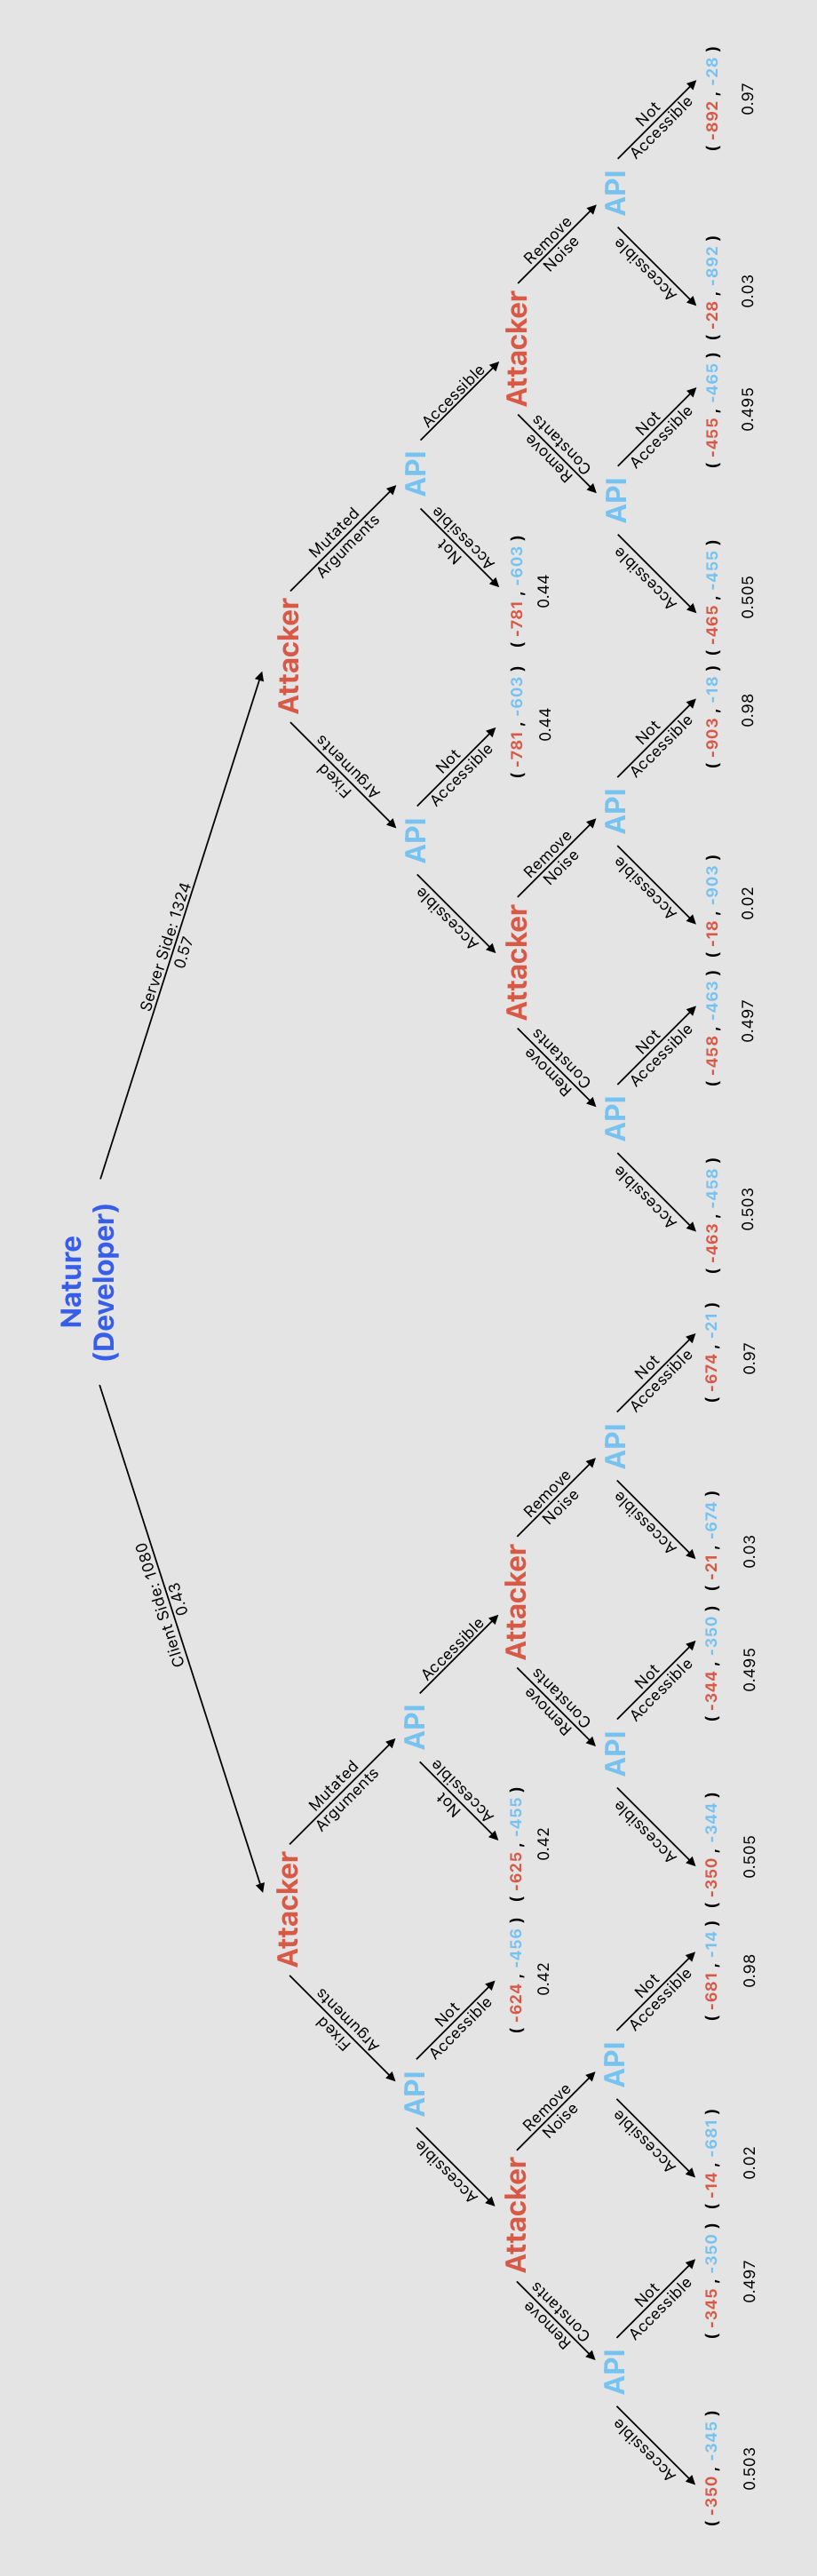
\includegraphics[width=3in,height=7.25in,keepaspectratio=FALSE]{graphics/api_game_tree_rotated.png}
    \caption{API Game Tree}
    \label{fig:api_game_tree}
\end{figure}

%%%%%%%%%%%%%%%%%%%%%%%%%%%%%%%%%%%%%%%%%
%%% Lab Task 2
%%%%%%%%%%%%%%%%%%%%%%%%%%%%%%%%%%%%%%%%%

\newpage

\section*{Task Set 2: Socially Engineer Application to Trick User and MPM}\label{sec:Task 2: Socially Engineer Application To Trick User And MPM}
\addcontentsline{toc}{section}{Task Set 2: Socially Engineer Application to Trick User and MPM}

\subsection*{Task 2.1: Tricking User}
\addcontentsline{toc}{subsection}{Task 2.1: Tricking User}

%\textbf{A. Background}
The idea behind social engineering is to convince and trick a suspected user into believing that an application is legitimate. If a service appears to be legitimate, it is much more likely a user will feel comfortable providing sensitive information to an attacker or an application. The technique behind this is through modeling an application as close as possible. Click the green play button at the top of the IDE and explore the device environment for yourself a little bit.

\bigskip
\begin{mdframed}[backgroundcolor=blue!10,style=code,nobreak=true,align=center,userdefinedwidth=14cm]

\textbf{Action}
\bigskip

2.1.1 - What common theme do you notice between some of the third-party applications installed on the device?\\
2.1.2 - What would be the best part or page of an application to mimic or trick a user and steal user information?\\
\end{mdframed}
\bigskip

If you notice, all of the third-party applications that are installed on our emulated device are shopping applications. Navigate to the log-in page of any one of these applications and take note of the layout. It is recommended that you take a screenshot of this page for future reference. An example of this is noted in figure~\ref{fig:example_login} Our first objective is to replicate this page within our application, and we will do so by learning about Android’s activity\_main.xml file that allows us to control and change the UI of our application. It is very similar in practice to HTML or JavaScript.

\begin{figure}[!h]
    \centering
    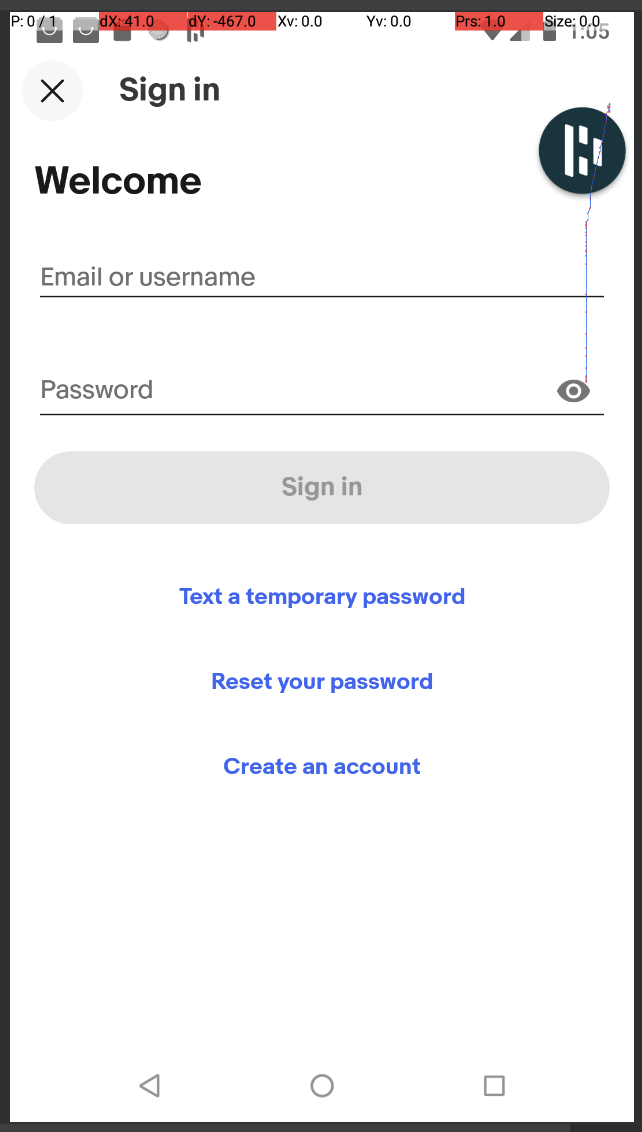
\includegraphics[width=0.4\columnwidth]{graphics/example_login.png}
    \caption{Example of login page}
    \label{fig:example_login}
\end{figure}

\bigskip
\bigskip
\bigskip
\bigskip
\bigskip
\bigskip
\bigskip
\bigskip
\bigskip
\bigskip
\bigskip
\bigskip
\bigskip
\bigskip


In your project window on the left-hand side, navigate to your 'res' package, and open the folder 'layout'. Beneath this, you will find your activity\_main.xml file. Once you open this, you will notice in the top right corner of your viewport that you have the option to change between your code and the design viewport. Here, you will implement any respective buttons, input fields, or images to match the log-in page from the target application as much as possible. You will notice that you have a skeleton outline for a few primitive operations to get you started on utilizing these features, but any additional features or solutions can be found on the~\href{https://developer.android.com/develop/ui}{Android Studio UI documentation}.

\bigskip
\begin{mdframed}[backgroundcolor=blue!10,style=code,nobreak=true,align=center,userdefinedwidth=14cm]
\textbf{Action}
\bigskip

2.1.3 - Create your replicated attack application and submit a screenshot of both your replicated version and the original application.
\end{mdframed}

\bigskip
\bigskip
\bigskip
\bigskip
\bigskip
\bigskip


\subsection*{Task 2.2: Stealing Credentials}
\addcontentsline{toc}{subsection}{Task 2.2: Stealing Credentials}

\begin{figure}[!h]
    \centering
    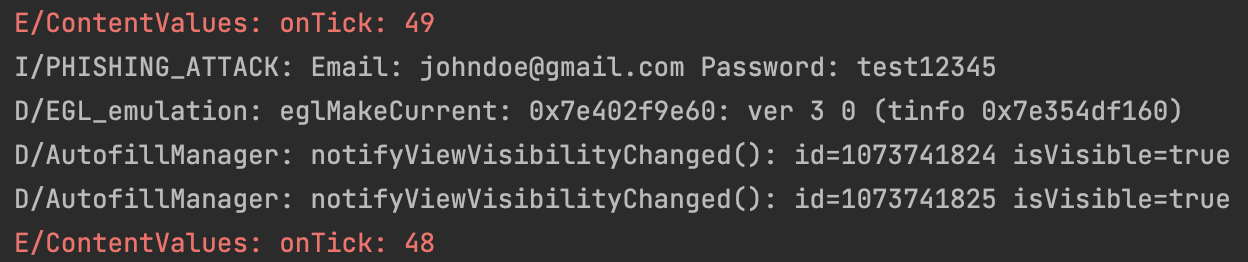
\includegraphics[width=1\columnwidth]{literature/stolen_credentials.png}
    \caption{Example of credentials stolen from application}
    \label{fig:stolen_credentials}
\end{figure}

Now that you have successfully created a page that could potentially trick a user, now it is time to trick the MPM into suggesting credentials and stealing them. Navigate back to your 'MainActivity.java' file. You will need to implement an~\href{https://developer.android.com/develop/ui/views/touch-and-input/input-events}{event listener} that will pull the credentials at an optimal time that were entered on your page, such as figure~\ref{fig:stolen_credentials}. This would typically be implemented after the 'log in' button is pressed. The trick to input fields and tricking the MPM is through a design tool known as ~\href{https://developer.android.com/guide/topics/text/autofill-optimize}{autofillHints}. Through your user-input fields, create a variable that will collect and store the inputs provided by the user and print them out to the console to validate that your method works. 

\bigskip
\begin{mdframed}[backgroundcolor=blue!10,style=code,nobreak=true,align=center,userdefinedwidth=14cm]

\textbf{Action}
\bigskip

2.2.1 - Create an input field within your 'activity\_main.xml' file that utilizes autofillHints to suggest what type of input to provide. Submit a screenshot of your element.\\
2.2.2 - Create an on click listener function within your 'MainActivity.java' class that steals credentials from the input field. Submit a screenshot of your code.\\
2.2.3 - Utilize the debug log to print out the stolen credentials to validate that your code performed as expected. Submit a screenshot of the output.\\
\end{mdframed}

%%%%%%%%%%%%%%%%%%%%%%%%%%%%%%%%%%%%%%%%%
%%% Task 3
%%%%%%%%%%%%%%%%%%%%%%%%%%%%%%%%%%%%%%%%%

\section*{Task Set 3: Accessing State Information Via Usage Stats Manager Through Background Service}\label{sec:Task 3: Accessing State Information Via Usage Stats Manager Through Background Service}
\addcontentsline{toc}{section}{Task Set 3: Accessing State Information via Usage Stats Manager Through Background Service}

\subsection*{Task 3.1: Permission for Usage Stats Manager}
\addcontentsline{toc}{subsection}{Task 3.1: Permission for Usage Stats Manager}

First things first - we need to provide our application access to the Usage Stats Manager. This section will teach you about~\href{https://developer.android.com/training/basics/intents/sending}{View Intents} and set you up for how to perform an injection in the next section. While it might seem silly to implement an attack that requires certain signature-level permissions, many real-world apps (both benign and malicious) currently use them, thus it is considered an appropriate threat model. First, it is smart for us to create a method that validates whether or not a permission has been previously provided as it will one improve the speed of our testing and two better trick the user into believing its validity once approved.

\begin{figure}[!h]
    \centering
    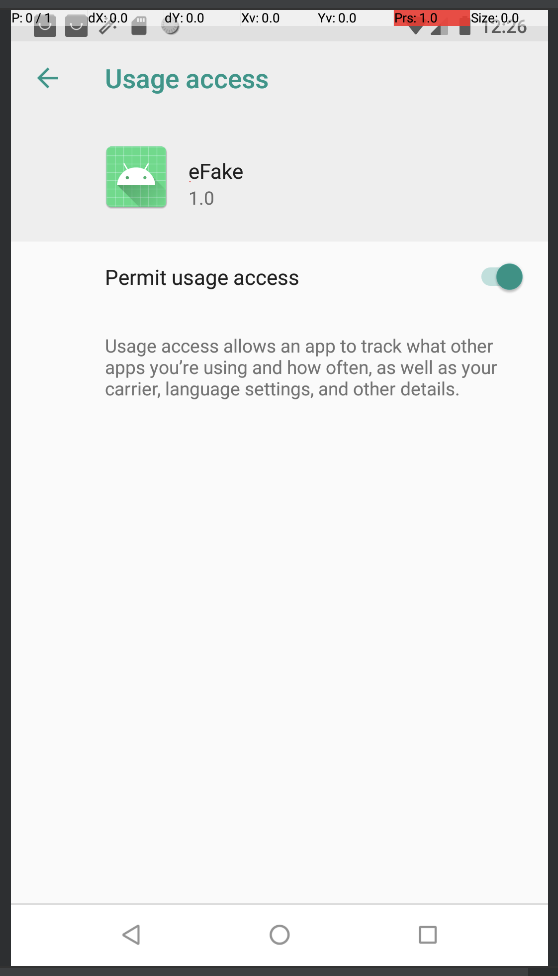
\includegraphics[scale=0.55]{graphics/permission_usm.png}
    \caption{Example of USM permission window}
    \label{fig:permission_usm}
\end{figure}

Navigate to 'MyService.java' and create a method at the start of your attack function within your runnable to check and see if the permission is granted as noted in figure~\ref{fig:permission_usm}. 

\bigskip
\begin{mdframed}
[backgroundcolor=blue!10,style=code,nobreak=true,align=center,userdefinedwidth=14cm]
\textbf{Action}
\bigskip

3.1.1 - Create a short section within 'MyService.java' that checks \\ whether or not Usage Stats Manager has been granted permission and submit a screenshot of your code.
\end{mdframed}

\bigskip

\subsection*{Task 3.2: Implementing Usage Stats Manager}
\addcontentsline{toc}{subsection}{Task 3.2: Implementing Usage Stats Manager}

\begin{figure}[!h]
    \centering
    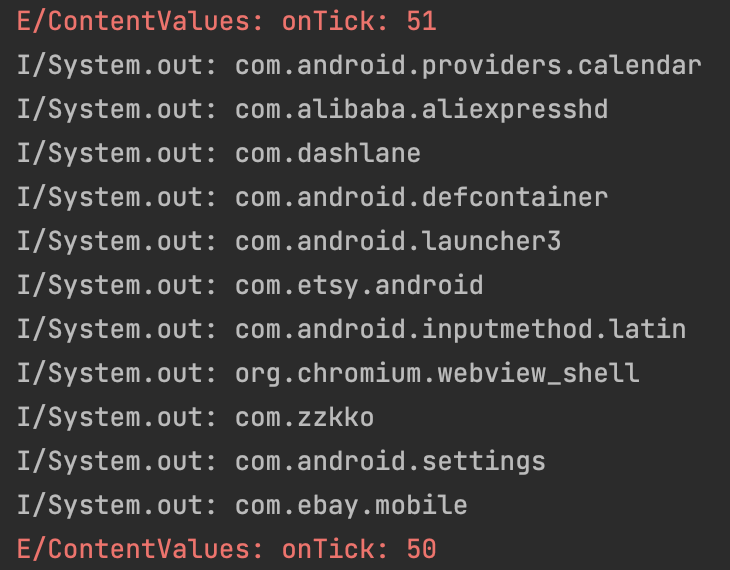
\includegraphics[scale=0.6]{graphics/usm_list.png}
    \caption{Example of USM package list}
    \label{fig:usm_list}
\end{figure}

Once you have enabled~\href{https://developer.android.com/reference/android/app/usage/UsageStatsManager}{Usage Stats Manager}, you will have access to the contained public methods that will allow you to access state information on the device. As you can see in figure~\ref{fig:usm_list}, this is an example output of active app packages in between tick intervals. Read through the short documentation notes and utilize one of the different public methods for Usage Stats Manager to return a list of information about all of the active packages. Note that each public method will return different types of information that can be used in a similar manner to determine state information. 

\bigskip

\begin{mdframed}[backgroundcolor=blue!10,style=code,nobreak=true,align=center,userdefinedwidth=14cm]
\textbf{Action}
\bigskip

3.2.1 - Now that you have permission to Usage Stats Manager, create a function that returns a list of activities and submit a screenshot of your code. Your output should be similar to Figure~\ref{fig:usm_list} on page~\ref{fig:usm_list} above.
\end{mdframed}

%%%%%%%%%%%%%%%%%%%%%%%%%%%%%%%%%%%%%%%%%
%%% Task 4: Game Theory
%%%%%%%%%%%%%%%%%%%%%%%%%%%%%%%%%%%%%%%%%

\section*{Task Set 4: Hijack Activity via View Intents Through Injection}\label{sec:Task 4: Hijack Activity Via View Intents Through Injection}
\addcontentsline{toc}{section}{Task Set 4: Hijack Activity via View Intents Through Injection}

Here, you will combine techniques learned in the previous modules to inject your activity. Through the list of services you identified via the Usage Stats Manager, choose a target application to monitor that is different than the application who's login page you selected to replicate. Do this by isolating the target application from the list returned from Usage Stats Manager and create conditional logic that identifies when that application is opened (in other words, moved to the foreground), and, using View intents, inject your application as if it were prompting the user to log in. Finally, once the user clicks the log in button on your replica page, utilize a separate View intent to return the user back to the original application they tried to open as if they never left it in the first place.

\bigskip

Furthermore, to convince the MPM that your application is legitimate, refactor your project to have an identical package name as the one you replicated. Thanks to increased security measures, Android prevents two applications from containing the same package name. By doing this, you will either replace or need to delete the previous application in order to successfully refactor your project. This is why it is even more important to replicate the original application as closely as possible. Do this by changing your applications package name to match your target application's package name within 'build.gradle (:app)' and 'AndroidManifeset.xml'. These can be found under the 'Gradle Scripts' and 'manifests' folders respectively beneath your project window. Once you've changed those, select 'File' -> 'Invalidate caches...' -> 'Restart', and your project should correctly rebuild. Note that you will likely have to reprovide permission to Usage Stats Manager, given that your application is considered a new app since it has a different package name.

\bigskip

\begin{mdframed}[backgroundcolor=blue!10,style=code,nobreak=true,align=center,userdefinedwidth=14cm]

\textbf{Action}
\bigskip

4.1.1 - Create a section that isolates your target application through monitoring the USM list and injects your malicious application via a view intent. Submit a screenshot of your code.\\
4.1.2 - Once you have injected your application, create a section that returns the user back to the target application after you've intercepted their credentials in a suspected 'log in' attempt. Submit a screenshot of your code.\\
\end{mdframed}

%%%%%%%%%%%%%%%%%%%%%%%%%%%%%%%%%%%%%%%%%
%%% Submission
%%%%%%%%%%%%%%%%%%%%%%%%%%%%%%%%%%%%%%%%%

\section*{Submission}\label{sec:Submission}
\addcontentsline{toc}{section}{Submission}

Submit a lab report utilizing the provided template to your instructor, which should include screenshots, thoughts, challenges, and lessons learned from the lab. Furthermore, zip and attach your project files with the relevant java files for submission.

%%%%%%%%%%%%%%%%%%%%%%%%%%%%%%%%%%%%%%%%%
%%% Summary
%%%%%%%%%%%%%%%%%%%%%%%%%%%%%%%%%%%%%%%%%

\section*{Summary}\label{sec:Summary}
\addcontentsline{toc}{section}{Summary}

This lab explored conventional attack strategies and mobile vulnerabilities to monitor and collect state information about a device. It also utilized social engineering and tools to trick a mobile password manager and user into providing sensitive information to be collected by an attacker.

\bigskip
\bigskip
\bigskip
\bigskip
\bigskip
\bigskip
\bigskip
\bigskip
\bigskip
\bigskip


\section*{Trouble Shooting}\label{sec:Trouble Shooting}
\addcontentsline{toc}{section}{Trouble Shooting}

\subsection*{MPM isn't recommending logins to save on certain devices/application}
\addcontentsline{toc}{subsection}{MPM isn't recommending logins to save on certain device/applications}

• Log into MPM and store the password combination yourself
    
\subsection*{Refactoring the Project Name}
\addcontentsline{toc}{subsection}{Refactoring the Project Name}

• Make sure you change the respective lines within build.gradle and AndroidManifest.xml to match what you refactored your project to. Then, select File->Invalidate Caches->Restart, and your project should rebuild with the correct dependencies. If this does not work, you can select Build->Clean Project and Build->Rebuild Project and then retry invalidating the caches. This will fully correct your problem.

\bibliography{References}
\bibliographystyle{plain}

\end{document}

%%%%%%%%%%%%%%%%%%%%%%%%%%%%%%%%%%%%%%%%%